\section{Coupling through preCICE}\label{sec:Coupl}
When a physical problem becomes too complex, one often split it into smaller pieces that are better manageable. These pieces, or physical fields, can then be solved separately and their solutions can be combined to an overall solution. This approach is called ``partitioned approach'' \cite{gatzhammer2015efficient}. This approach allows to reuse the simulation code for the single fields and simultaneously provides the possibility to encapsulate the coupling functionality itself as a reusable component, too. This allows minimal access to solver codes, i.e., treating them as black boxes. At the same time the solver code does not have to include the whole coupling code making it less application dependent. The coupling tool preCICE offers coupling functionality to develop a multi-physics simulation environment using existing solvers. In this work a fluid-structure interaction (FSI) will be simulated. The thesis' program represents the structure part whereas the fluid part can be dynamically exchanged due to the coupling with preCICE. This Chapter gives an overview of preCICE and its main components and shows the implementation modifications that were necessary to integrate preCICE and prepare the code for coupling.

 \subsection{Overview of preCICE}\label{sec:Coupl-OverviewPreCICE}
  The goal of preCICE is to provide all functionality to realize a multi-physics simulation environment working with existing single-physics solvers. This includes simulations like fluid-structure, fluid-acoustics, fluid-solid thermodynamics and porous-free flow interactions, for instance. It provides technical inter-code communication via MPI or TCP/IP, methods for data mapping between different grids and coupling methods based on quasi-Newton methods to ease the development process. preCICE supports parallel solvers through efficient point-to-point communication without the need of a server instance. It also features a high-level API making its integration into existing solver code minimal invasive \cite{bungartz2015fully}.
  
  preCICE supports partitioned coupling of black box solvers with focus on FSI and provides a geometry interface for Cartesian grid solvers. Its API is available for C++, C, and Fortran and consists of high-level methods enabling solvers to use coupling functionality in a flexible way. After the preCICE integration into the solver's code, a peer-to-peer communication without central control instance is generated. The single solver codes can be run serial or parallel without major modifications to the integrated API. Furthermore, the concrete coupling algorithms in the simulation can be selected through an XML configuration file that optimizes the solver adaption \cite{gatzhammer2015efficient}.
  
  \begin{figure}[htbp]
  	\centering
  	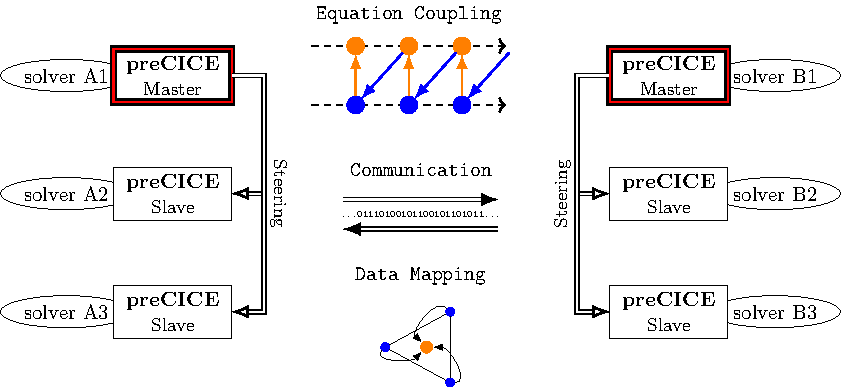
\includegraphics[width=0.97\linewidth]{figures/NewCommunicationScheme}
  	\caption{Schematic view of a partitioned multi-physics simulation with two solvers (A and B) coupled through preCICE. In the middle are the three main functionalities of preCICE shown, that steer coupling iterations: Fix-point acceleration methods, point-to-point communication and data mapping between non-matching grids at the coupling interface. Picture courtesy of Florian Lindner \cite{bungartz2015fully} }
  	\label{fig:precice}
  \end{figure}
  
  Figure \ref{fig:precice} shows a schematic view of the main functionality groups of preCICE. Two solvers (A and B) are coupled through the preCICE tool. The three main functionalities of preCICE are drawn in the middle: Fix-point acceleration methods, point-to-point solver process communication and data mapping between non-matching grids at the coupling surface. Each shown solver runs in parallel with a master process controlling tasks such as convergence for the corresponding solver as well as for the whole simulation. The following sections describe each of the three addressed main functionalities in greater detail.
  
 
 \subsection{Coupling Methods}\label{sec:Coupl-Coupling}
  preCICE distinguishes two possible coupling schemes: Explicit and implicit coupling. A single time step of multi-physics simulation partitioned into several solvers can be done with only a small and fixed number of calls of time steps per solver. This is described by an explicit coupling scheme. The alternative is an iterative procedure that achieves convergence with respect to the monolithic solution of the system in each time step. An implicit coupling scheme then iterates over a coupling equation until convergence occurs. Based on \cite{bungartz2015fully} it is assumed that two solvers $S_1$ and $S_2$ make up a coupled system. Vector spaces $X_1$ and $X_2$ describe data at the coupling interface to be mapped between the two solvers in a single time step. The output of $S_1$ is required as an input by $S_2$ and vice versa, i.e. it follows:
  \begin{equation}
  S_1: X_1 \leftarrow X_2\quad \text{and}\quad S_2:X_2 \leftarrow X_1
  \end{equation}
  The fluid-structure coupling done in this work, is an example for a Dirichlet-Neumann type coupling. The displacements at the coupling interface of the structure solver is the input for the fluid solver that gives forces to the structure solver as its output.
 
  \subsubsection{Explicit Coupling Schemes}\label{sec:Coupl-Coupling-Explicit}
   Two different implementations of explicit coupling schemes exist in preCICE: The staggered scheme and the parallel scheme. The staggered scheme uses the old time step's values $x_1^{(n)}$ at the coupling surface for the execution of the $n$th time step ($t_n \leftarrow t_{n+1}$) to achieve $x_2^{(n+1)}$. These new values act as boundary values for the $n$th time step of $S_2$ \cite{bungartz2015fully}:
   \begin{equation}
   x_2^{(n+1)} = S_1^{(n)}\left( x_1^{(n)} \right)\quad \text{and}\quad x_1^{(n+1)} = S_2^{(n)}\left( x_2^{(n+1)} \right)
   \end{equation}
   Since the two solvers are executed staggered, this scheme is not optimal with respect to load balancing \cite{bungartz2015fully}. In contrast, the parallel scheme does not have this drawback. It uses the old time step values $x_1^{(n)}$ and $x_2^{(n)}$ as inputs for both solvers:
   \begin{equation}
   x_2^{(n+1)} = S_1^{(n)}\left( x_1^{(n)} \right)\quad \text{and}\quad x_1^{(n+1)} = S_2^{(n)}\left( x_2^{(n)} \right)
   \end{equation}
   According to \cite{bungartz2015fully} both explicit schemes yield consistent time steps but cause instabilities that cannot be avoided, even if the time step length is reduced.
  
  \subsubsection{Implicit Coupling Schemes}\label{sec:Coupl-Coupling-Implicit}
   All implicit coupling schemes in preCICE are based on fixed-point iterations using the staggered or the parallel explicit scheme. The fixed-point iteration regarding the staggered scheme is as follows:
   \begin{equation}
   x_2^{(n+1),i+1} = S_1^{(n)}\left( x_1^{(n+1),i} \right)\quad \text{and}\quad x_1^{(n+1),i+1} = S_2^{(n)}\left( x_2^{(n+1),i+1} \right)
   \end{equation}
   The fixed-point iteration corresponding to the parallel scheme can be written as:
   \begin{equation}
   x_2^{(n+1),i+1} = S_1^{(n)}\left( x_1^{(n+1),i} \right)\quad \text{and}\quad x_1^{(n+1),i+1} = S_2^{(n)}\left( x_2^{(n+1),i} \right)
   \end{equation}
   Here, the new iterates for $x_2^{(n+1),i+1}$ and $x_2^{(n+1),i+1}$ are computed in parallel. preCICE offers simple underrelaxation, adaptive Aitken underrelaxation and various quasi-Newton solvers in order to solve these fixed-point equations in as robust and stable as possible \cite{bungartz2015fully}. In the following a generic fixed-point equation
   \begin{equation}\label{eq:fixed-point-eq}
   x = H(x)
   \end{equation}
   is considered. Every fixed-point equation solver in preCICE is a combination of a fixed-point iteration and a post-processing step that modifies the result of the fixed-point iterator. Underrelaxed fixed-point iterations are the simplest solvers \cite{bungartz2015fully}:
   \begin{equation}
   x^{i+1} = H(x^i)+(\omega - 1)\left( H(x^i) - x^i\right)
   \end{equation}
   with $\omega \in \mathbb{R}, 0 < \omega \leq 1$ either a user-defined value or additionally adapted by the solver throughout the iterations using Aitken underrelaxation.
   In order to get the full potential of a parallel scheme, preCICE provides a powerful class of convergence acceleration methods, called quasi-Newton methods. With these methods a fast convergence is achieved in particular for difficult problems when using parallel fixed-point iterations \cite{bungartz2015fully}. All quasi-Newton methods in preCICE accelerate the fixed-point iteration by a subsequent Newton step \cite{bungartz2015fully}:
   \begin{align}
   x^{k+1} = \underbrace{H(x^k)} - J_{\tilde{R}}^{-1}\left( \underbrace{H(x^k) - x^k}\right) \\
   =: \tilde{x}^k\qquad =\tilde{x}^k - H^{-1}(\tilde{x}^k) \nonumber
   \end{align}
   where $\tilde{R} = I-H^{-1}$ maps $\tilde{x}^k$ to the residual $r^k=\tilde{R}(\tilde{x}^k)=H(x^k)-x^k$. The inverse of the Jacobian $J_{\tilde{R}}^{-1}$ can be approximated ($\hat{J}_{\tilde{R},k}^{-1}$) in different ways in preCICE:
   \begin{itemize}
   	\item The classical interface quasi-Newton (IQN) approach uses the approximated inverse Jacobian with minimal Frobenius norm:
   	\begin{equation}
   	\left\| \hat{J}_{\tilde{R},k}^{-1} \right\|_F \leftarrow \min
   	\end{equation}
   	\item The multi-vector quasi-Newton (IMVJ) approach minimizes the distance between $\hat{J}_{\tilde{R},k}^{-1}$ and the approximate $\hat{J}_{\tilde{R},k}^{-1,(n)}$ from the last time step:
   	\begin{equation}
   	\left\| \hat{J}_{\tilde{R},k}^{-1} - \hat{J}_{\tilde{R},k}^{-1,(n)}\right\|_F \leftarrow \min
   	\end{equation}
   \end{itemize}
   For more details, see \cite{bungartz2015fully} and \cite{gatzhammer2015efficient}.
   
   Additional specifications can be made by the user to adapt the coupling method to the problem. A statement of extrapolation in time can be made to get a better initial guess for the next time step solution and with subcycling several small time steps are done in one of the solvers while the others use a larger time step.
  

 \subsection{Data Mapping} \label{sec:Coupl-DataMapping}
  Due to the fact that independent solvers are used for coupling, it can happen that the single solver meshes are non-matching. This requires a mapping of the data that is sent by the above iterative coupling methods from the coupling surface of one solver domain to the surface of the other solver domain. The case where the two meshes matching each other is not very common when dealing with two distinct solvers and would only result in a copying of data values for transfer without any interpolation or projection. In the case of non-conforming meshes interpolation algorithms are necessary and when the two grids overlap or gaps exist even projections in some form are additionally required \cite{gatzhammer2015efficient}. preCICE offers some data mapping methods but also provides the possibility for user-defined mapping implementations for special needs \cite{bungartz2015fully}.
  \subsubsection{Conservative vs.\ Consistent}\label{sec:Coupl-DataMapping-conVScon}
   The mapping of displacements and pressures, for example, usually requires a \textbf{consistent mapping}, i.e. constants should be interpolated exactly. Let $\underline{H}_{AB} \in \mathbb{R}^{n_A \times n_B}$ be the matrix mapping values between variables from solver $A$ to $B$. Then consistent mapping can be expressed as follows:
   \begin{equation}
   \underline{\beta}_B = \underline{H}_{AB} \underline{\beta}_A
   \end{equation}
   with the arbitrary variable $\beta$ whose values are represented as matrix $\beta_{A,i} = \beta_{B,j} = \beta = const, 1 \leq i \leq n_A, 1 \leq j \leq n_B$. The property of exact constant interpolation is the case if and only if the row sums of the mapping matrix are equal to 1 \cite{gatzhammer2015efficient}:
   \begin{equation}
   \beta_{B,i} = \sum_{j=1}^{n_A} H_{AB,ij}\beta_{A,j} = \beta_{A,j} = \beta \qquad \forall i
   \end{equation}
   
   A \textbf{conservative mapping} on the other hand is important for integral values like forces. This mapping approach requires the sum of the data values is equal on both sides:
   \begin{equation}
   \sum_{i=1}^{n_B}\beta_{B,i} = \sum_{j=1}^{n_A}\beta_{A,j}
   \end{equation}
   This property holds only for the column sums of $\underline{H}_{AB}$ to be equal to 1:
   \begin{equation}
   \sum_{i=1}^{n_B}\beta_{B,i} = \sum_{i=1}^{n_B}\left( \underline{H}_{AB}\underline{\beta}_A \right)_i = \sum_{i=1}^{n_B}\sum_{j=1}^{n_A} H_{AB,ij}\beta_{A,j} = \sum_{j=1}^{n_A}\left( \sum_{i=1}^{n_B} H_{AB,ij}\right) \beta_{A,j} = \sum_{j=1}^{n_A} 1 \beta_{A,j}
   \end{equation}
   Further details to the mathematical background of the two mapping approaches can be found in \cite{gatzhammer2015efficient}. Both mappings are available for all methods described below.

  \subsubsection{Nearest-Neighbor}\label{sec:Coupl-DataMapping-NN}
   The Nearest-Neighbor mapping method works locally and requires only vertex positions, i.e. only the data nodes of the solver surface meshes are required for the mapping. The mapping itself is simple: In order to map values from mesh A to mesh B, for every node of mesh B the geometrically closet neighbor to a node of mesh A needs to be determined. Then, the data value from the closest node in mesh A is copied to the corresponding node in mesh B. There are special cases that can happen with this projection method: A value from mesh A can be copied to more than one node of mesh B if the node in mesh A is closest to all of the B nodes. On the other hand, nodes in A can be omitted if no projection partner in B were found, since the search for nearest neighbors is done on mesh B only. This is a general problem of all projection methods \cite{gatzhammer2015efficient}.
   
   If the meshes have matching vertex positions then this mapping method is good choice. For non-conforming meshes the first order accuracy of Nearest-Neighbor makes it a rather bad choice and other mapping methods should be taken into account \cite{bungartz2015fully}.
  
  \subsubsection{Nearest-Projection}\label{sec:Coupl-DataMapping-NP}
   The Nearest-Projection mapping requires not only vertex positions but also topology information for the source mesh. It searches for mesh nodes on the target mesh and creates geometrical projections to a matching set of elements on the source mesh. An interpolation is employed from nodes to mesh elements and vice versa. The finding of closest neighbors is similar to Nearest-Neighbor, but Nearest-Projection uses faces instead of points for its projections and several data nodes can be involved \cite{gatzhammer2015efficient}. Just as for the Nearest-Neighbor mapping, nodes can be omitted here if the mesh widths differ too much locally and theoretically this method is also of first order due to the projection. In practice, due to the fact that often the distance between the two meshes normal to the coupling interface is smaller that the mesh widths, a second order accuracy can be observed \cite{bungartz2015fully}.
  
  \subsubsection{Radial Basis Function}\label{sec:Coupl-DataMapping-RBF}
   This mapping method uses radial basis functions (RBF) centered at the mesh nodes of the source mesh. It does not require topological information, projections or search-algorithms. It works well on general non-conforming meshes, where overlapping meshes or gaps between them can occur. Several different basis functions are implemented in preCICE, including Gaussian, (Inverse) Multiquadrics, Thin Plate Splines, Volume Splines (see \cite{bungartz2015fully}), but further functions can be added easily. The global support of some RBFs (Gaussian and Thin Plate, for instance) can be limited to a smaller area by introducing a cut-off radius. This reduces the density of the system matrix for interpolation and thus reduces the amount of communication between the solvers and the computational complexity of the data mapping. This allows local communication while still having the properties of the radial basis functions \cite{bungartz2015fully}.


 \subsection{Communication} \label{sec:Coupl-Communication}
  The coupling of different solvers in the frame of a multi-physics simulation requires an efficient communication between different executables. preCICE offers a communication per interaction of two or more participants. Either MPI ports or low level TCP/IP sockets are available for communication in preCICE. A fully parallel point-to-point data transfer is possible with preCICE, since it analyses the mesh decomposition of all participants and constructs only local communication channels where they are needed \cite{bungartz2015fully}.
 
  \subsubsection{MPI Communication}\label{sec:Coupl-Communication-MPI}
   The message passing interface (MPI) is used in preCICE with a multiple program multiple data paradigm, i.e. two different codes are communicating with their own data. Two MPI-based communication methods are implemented which differ in the way how they set up the communication space. With the first method all executables are put in the same communication space, called ``communicator world''. All processes of each participant are then grouped into separate communicators. An inter-communicator is used as the actual channel for data exchange.
   The second method establishes a connection between processes started individually and in different communication spaces. The exchange of connection information is done through a commonly accessible file which stores the port names of the participants. For this a MPI version of 2 or greater is needed \cite{gatzhammer2015efficient}. The result is the same as with method one: An inter-communicator.
   
  \subsubsection{Socket Communication}\label{sec:Coupl-Communication-TCP}
   The communication by TCP/IP increases compatibility to closed-source software that might be restricted to some MPI implementations \cite{bungartz2015fully}. To abstract from platform dependent socket interfaces like Pthreads or Winsock, the Boost.Asio (asynchronous network and low-level input/output) library was used for implementing the socket communication in preCICE \cite{gatzhammer2015efficient}. The sending and receiving of data is managed by the transfer control protocol (TCP) which is designed for failsafe data transfer and synchronization between sender and receiver. Communication via TCP is not typical for multi-physics simulations that often run on supercomputers, because it involves a synchronization step and additional communication overhead compared to MPI. Other difficulties are that ports used for socket communication may be blocked by default and each supercomputer node might have different network address which requires automated checks on a low-level socket layer \cite{gatzhammer2015efficient}.


 \subsection{Implementation}\label{sec:Coupl-Impl}
  The program developed in the scope of this thesis is to be coupled with a fluid solver in a fluid-structure interaction simulation. The coupling is done with the help of preCICE. This section contains the steps that were necessary to adapt the original code to preCICE, including a general preCICE integration example, the introduction of additional boundary conditions, the partitioning of the coupling surface and the actual API integration details.
  
  
  \subsubsection{preCICE Code Example}\label{sec:Coupl-Impl-Example}
   One goal of preCICE is that its API can be integrated into existing solver code with minimal modifications to the original solver in order to make it part of a multi-physics coupled simulation. Listing \ref{lst:preCICEex} shows an integration example of preCICE into an arbitrary solver code. The main parts of the preCICE code are: The creation of the interface object in line 3 and the loading of the XML-configuration file the line below, the setup of the interface structures (line 5-7), the while-loop that is executed as long as the simulation has not finished (line 13) and the exchange of data in line 19 and 21). The call of the \texttt{precice.advance}-function (line 20) executes the preCICE coupling numerics, interpolations and communications, as stated in the previous sections. More details on the single preCICE steps are described in the following when the actual preCICE integration into the thesis' program code is shown.
\begin{lstlisting}[caption=preCICE Integration Example,label=lst:preCICEex,keepspaces=true]
// ... solver specific initialization steps

precice::SolverInterface precice("SolverName", solverRank, solverThreadSize);
precice.configure("precice-config.xml");
int dataID = precice.getDataID("DataName");
int* vertexIDs = new int[n_nodes];
precice.setMeshVertices(meshID, dataSize, coordinates, vertexIDs);

// ... setup solver data structures like forces, displacements, etc.

double preciceMaxDt = precice.initialize();

while (precice.isCouplingOngoing())
{
	dt = min(preciceMaxDt, solverDt);

	// ... computer solver time step

	precice.writeBlockVectorData(dataID, dataSize, dataIndices, data);
	preciceMaxDt = precice.advance(dt);
	precice.readBlockVectorData(dataID, dataSize, dataIndices, data);
}

precice.finalize();
// ... solver specific finalization steps
\end{lstlisting}
   
  \subsubsection{Additional Boundary Conditions}\label{sec:Coupl-Impl-BCs}
   When the solver is coupled to another solver, a part of (or the whole) mesh is acting as the interface surface to the other side. preCICE uses this coupling interface to exchange the data values between the two sides. In order to be flexible with respect to the fluid solver part, this interface region is to be defined arbitrarily within the mesh file that is imported by the structure solver. The definition which node is part of the coupling interface and which not, is done by a separate boundary condition ID. This guarantees no additional modifications to the mesh import since only the mesh files itself needs to be changed accordingly. Such modified files can even be used without the coupled version of the solver as the added boundary conditions will simply be ignored by the stand-alone version of the solver.
   
   The structure solver accepts two different types of boundary conditions in the unmodified version: Simply supported (ID=0) and clamped (ID=1). These are defined at the mesh's boundary in general. With the coupling update three more boundary condition IDs are required:
   \begin{itemize}
  	\item \textbf{\texttt{2}}: A node with this ID is defined to be part of the preCICE coupling interface. It can be positioned at the mesh's boundary or within the mesh.
  	\item \textbf{\texttt{20}}: Such a node has a simply supported boundary condition \textbf{and} is additionally part of the coupling interface. This ID is necessary since the boundary condition is required by the structure solver to work correctly and the coupling interface definition is required by preCICE to exchange data at this node with the fluid solver.
  	\item \textbf{\texttt{21}}: Here, the node has a clamped boundary condition \textbf{and} is part of the coupling interface. The reason for this ID is the same as for the above.
   \end{itemize}
   
   The new definitions adds only two more lines to the original code, as can be seen in Listing \ref{lst:addBoundary}. LibMesh uses a ``set'' data structure to be able to assign multiple different IDs to one \texttt{DirichletBoundary}-object which is exactly needed here.
\begin{lstlisting}[caption=Additional boundary condition IDs,label=lst:addBoundary,keepspaces=true]
// (...)
std::set<boundary_id_type> boundary_ids;
boundary_ids.insert(0);
boundary_ids.insert(20); // NEW
// (...)
boundary_ids.clear();
boundary_ids.insert(1);
boundary_ids.insert(21); // NEW
// (...)
\end{lstlisting}
  	
  \subsubsection{Partitioned Coupling Surface}\label{sec:Coupl-Impl-PartCplSurf}
   As stated in the section above, preCICE expects a coupling interface region on the structure solver's mesh. The definition of this region happens in the mesh file that is imported by the solver at the beginning of the simulation. The solver stores the mesh as an internal libMesh \texttt{Mesh}-object. For the interface region, an own grid-like structure needs to be defined that stores the vertex positions of the region's nodes. Listing \ref{lst:partCplSurf} is an extract of the coupled program code. First, an advantage of libMesh and preCICE can be seen in line 3 and 4: The code is usable with and without MPI without any code modifications: With the usage of the prefix ``local'' for the node iterators, every MPI process only searches its own mesh partition for coupling interface nodes. If no MPI is used, local is equal to global and the only existing process goes through all mesh nodes. On the other hand does preCICE not distinguish between a serial or parallel solver code - although it handles parallel solvers different to serial solvers internally (see \cite{gatzhammer2015efficient}).
   
\begin{lstlisting}[caption=Partition Coupling Surface,label=lst:partCplSurf,keepspaces=true]
// (...) preCICE successfully configured
MeshBase::const_node_iterator           no = mesh.local_nodes_begin();
const MeshBase::const_node_iterator end_no = mesh.local_nodes_end();
int n_nodes = 0;
BoundaryInfo info = mesh.get_boundary_info();
info.build_node_list_from_side_list();
std::vector<const Node*> preCICEnodes;
for (; no != end_no; ++no)
{
	const Node *nd = *no;
   	if (info.has_boundary_id(nd,2)  ||
	    info.has_boundary_id(nd,20) ||
	    info.has_boundary_id(nd,21))
   	{
	   	preCICEnodes.push_back(nd);
   	}
}
n_nodes = preCICEnodes.size();
int dimensions = interface.getDimensions();
double* grid = new double[dimensions * n_nodes];
// (...)
std::vector<const Node*>::iterator iter = preCICEnodes.begin();
for (int i = 0; iter != preCICEnodes.end(); ++iter,++i)
{
	const Node *nd = *iter;
	// (...)
	grid[i*dimensions]   = (*nd)(0);
	grid[i*dimensions+1] = (*nd)(1);
	grid[i*dimensions+2] = (*nd)(2);
}
// (...)
int meshID  = interface.getMeshID("Structure_Nodes");
int *vertexIDs = new int[n_nodes];
interface.setMeshVertices(meshID, n_nodes, grid, vertexIDs);
\end{lstlisting}

   In line 6 of Listing \ref{lst:partCplSurf} a \texttt{BoundaryInfo}-object is created. This class contains information relevant to boundary conditions, since it can mark element faces and nodes with IDs useful for identifying the type of boundary condition. The next line is needed when a mesh file written in the libMesh-format XDR/XDA was imported. In such a file the boundary conditions can only be defined at element's sides. The \texttt{BoundaryInfo}-object then contains only information regarding edges, not nodes. The function called in line 7 applies these information to the mesh nodes, too, such that the boundary condition IDs can be asked from the node. The for-loop between line 9 and 18 goes through all local nodes of the mesh partition. Inside of it, it is checked whether the current node has a boundary condition ID that defines it to be part of the coupling interface. If so, a pointer to this node is stored in a vector for further processing. After the for-loop the number of nodes of the interface part is saved.
   
   After it is known how many and which nodes are part of the coupling interface, the grid-like structure needs be created and filled. This is done in line 21 and 24 to 31. An array of \texttt{double}-values represents the structures. It has $dimensions * n_nodes$ entries. preCICE expects the ordering to be as follows: $p_{1_x}, p_{1_y}, p_{1_z}, p_{2_x}, \ldots, p_{n_y}, p_{n_z}$, with $p_i$ being the $i$th node defined in 3D space. The for-loop beginning in line 24 simply iterates over the earlier stored nodes and assigns its geometrical positions to the corresponding entries in the grid-structure.
   
   preCICE holds an ID for every mesh a solver contributes to the coupled simulation. The ID of the structure mesh is get from preCICE is line 32. Additionally, preCICE holds an internal representation of the vertices of the coupling interface. Every such a vertex has a globally (throughout the solvers) valid ID. These IDs may be different to the node IDs of the structure mesh. For the data exchange with preCICE to function properly the IDs must be get from preCICE. This is done in line 33 and 34. According to the single geometric vertex positions, preCICE find the corresponding internal vertex and returns its ID.

  \subsubsection{Integration of preCICE}\label{sec:Coupl-Impl-Integration}
   The changes in the mesh import and the creation of the coupling interface partitions were preprocessing steps that laid the foundation of the actual preCICE integration into the solver code. Before any preCICE function can be used, a \texttt{SolverInterface}-object of preCICE must be created with the name of the solver, the ID of the calling process and the overall number of processes used for this solver (see Listing \ref{lst:preCICEint1}). Next, the XML-configuration file must be loaded on configured by preCICE.
\begin{lstlisting}[caption=preCICE Integration Part 1,label=lst:preCICEint1,keepspaces=true]
// (...) libMesh Initialization and mesh import
SolverInterface interface(solverName, global_processor_id(), global_n_processors());
interface.configure(config_filename);
\end{lstlisting}
   The structure solver in its current state gets forces as input from the fluid solver and produces displacements as output sent back to the fluid solver. In order to accelerate the data exchange, all data is sent at once and received at once. Therefore, in Listing \ref{lst:preCICEint2} two arrays are created (line 1 and 2) with as many entries as the process owns nodes of the coupling interface multiplied by the number of dimensions (typically 3). These variables were defined by the XML-configuration file, too and present in preCICE. For the data exchange their IDs must be get from preCICE, which is done in line 5 and 6. Inside the for-loop that also fills the grid-like structure from Listing \ref{lst:partCplSurf} with vertex position, initial values for the displacements and forces are set. This must be done by one of the coupled solvers; which one is defined in the XML-configuration file.

\begin{lstlisting}[caption=preCICE Integration Part 2,label=lst:preCICEint2,keepspaces=true]
double *displ = new double[dimensions*n_nodes];
forces = new double[dimensions*n_nodes];
// (...)
int meshID  = interface.getMeshID("Structure_Nodes");
int displID = interface.getDataID("Displacements", meshID);
int forceID = interface.getDataID("Forces", meshID);
// (...)
for (int i = 0 ; iter != preCICEnodes.end(); ++iter,++i)
{
	const Node *nd = *iter;
	for (int dims = 0; dims < dimensions; dims++)
	{
		displ[i*dimensions+dims]  = 0.0;
		forces[i*dimensions+dims] = 0.0;
	}
	// (...)
}
\end{lstlisting}
   As stated in section \ref{sec:Coupl-Impl-PartCplSurf}, the vertex IDs of preCICE does not necessarily match the IDs of the structure's mesh node IDs. To be able to apply the correct forces to the correct mesh nodes, a mapping must be performed. Listing \ref{lst:preCICEint3} displays this in the lines 1 to 6: A for-loop iterates over the coupling interface nodes and stores the linking of the mesh nodes IDs to the preCICE vertex IDs in a \texttt{std::unordered\_map}-data structure which is efficient in adding elements and finding them later. The \texttt{id\_map} is used when the right-hand side of the single elements is generated and described in further details in Listing \ref{lst:preCICE-contribRHS}.

\begin{lstlisting}[caption=preCICE Integration Part 3,label=lst:preCICEint3,keepspaces=true]
iter = preCICEnodes.begin();
for (int i = 0 ; iter != preCICEnodes.end(); ++iter,++i)
{
	std::pair<dof_id_type, int> pair( (*iter)->id(), vertexIDs[i] );
	id_map.insert(pair);
}

interface.initialize();
if ( interface.isActionRequired(actionWriteInitialData()) )
{
	interface.writeBlockVectorData(displID, n_nodes, vertexIDs, displ);
	interface.fulfilledAction(actionWriteInitialData());
}
interface.initializeData();
if ( interface.isReadDataAvailable() )
	interface.readBlockVectorData(forceID, n_nodes, vertexIDs, forces);

// (...) libMesh equation system setup etc.
\end{lstlisting}
   With line 8 preCICE gets finally initialized. The lines 9 to 13 performs sends the initial data set in Listing \ref{lst:preCICEint2}) to preCICE. The call in line 14 tells preCICE to communicate all initial data to every solver, including the calling one. In line 16 possible available initial force values are read.
   
   Listing \ref{lst:preCICEint4a} contains the main while-loop that is executed until the complete simulation is finished (\texttt{isCouplingOngoing()}) or a critical error happened which quit the simulation, too. The lines 3 and 4 are only required when an implicit coupling scheme was chosen in the preCICE configuration. This requires so-called ``Checkpoints'' to be created. Since the coupled solvers are only sub-components of the overall simulation, they cannot access all information needed to control the simulation. preCICE is the control instance that decides what kind of computation step has to be performed next by a solver. This includes the responsibility for synchronized writing of outputs on the convergence of a time step or restarting a simulation step. For this, the old time step state needs to be saved and this is realized by checkpoints. If a checkpoints is written to or read from is managed by preCICE and the solver only do it when the corresponding action is required.
   
   In line 6 the linear elastic problem with the given mesh and forces is solved by the program. As addressed in section \ref{sec:Impl-Details-Solving} the solution is only accessible for the master process. In the stand-alone version of the program this was not a problem, because the master process could have write the output into a file or put it onto the console. When the program is part of a coupled simulation, every single process must tell preCICE its own displacements. After building the solution vector in line 9, a broadcasting of the results must be performed: Every non-master process reserves enough space in its solution vector to store the data. The master process broadcasts its solution to the other processes. If the program is not executed in parallel this step is ignored by the two if-clauses. When every process got the solution, they can assign them to displacements to the array that is used for data exchange.
   
\begin{lstlisting}[caption=preCICE main while-loop part 1,label=lst:preCICEint4a,keepspaces=true,name=while-loop]
while ( interface.isCouplingOngoing() )
{
	if ( interface.isActionRequired(actionWriteIterationCheckpoint()) )
		interface.fulfilledAction(actionWriteIterationCheckpoint());

	equation_systems.solve();

	std::vector<Number> sols;
	equation_systems.build_solution_vector(sols);
	if (global_processor_id() > 0)
		sols.reserve(mesh.n_nodes()*6);
	if (global_n_processors() > 1)
		mesh.comm().broadcast(sols);

	std::vector<const Node*>::iterator iter = preCICEnodes.begin();
	for (int i = 0 ; iter != preCICEnodes.end(); ++iter,++i)
	{
		int id = (*iter)->id();
		displ[i*dimensions]   = sols[6*id];
		displ[i*dimensions+1] = sols[6*id+1];
		displ[i*dimensions+2] = sols[6*id+2];
	}
\end{lstlisting}
   In the lines 23 and 25 the actual data exchange is taken place. First the solver writes its solution to preCICE. Then the \texttt{advance}-function of preCICE is called with a parameter that represents the actually used time step length of the solver. The function updates the coupling state, maps data between non-matching grids and exchanges data between the coupled solvers. Further, it applies iteration acceleration schemes (cf. \ref{sec:Coupl-Coupling-Implicit}) and measures the convergence of coupling iterations when implicit coupling is used (like in this case) \cite{gatzhammer2015efficient}. In line 25 the new force values are read and assigned to the corresponding array.

\begin{lstlisting}[caption=preCICE main while-loop part 2,label=lst:preCICEint4b,keepspaces=true,name=while-loop]
	interface.writeBlockVectorData(displID, n_nodes, vertexIDs, displ);
	interface.advance(dt);
	interface.readBlockVectorData(forceID, n_nodes, vertexIDs, forces);

	if (interface.isActionRequired(actionReadIterationCheckpoint()))
		interface.fulfilledAction(actionReadIterationCheckpoint());
	else
	{
		t++;
		if (global_processor_id() == 0)
		{
			MeshBase::const_node_iterator no = mesh.nodes_begin();
			const MeshBase::const_node_iterator end_no = mesh.nodes_end();
			for (int i = 0 ; no != end_no; ++no,++i)
			{
				Node *nd = *no;
				(*nd)(0) += sols[6*i];
				(*nd)(1) += sols[6*i+1];
				(*nd)(2) += sols[6*i+2];
			}
		}
	}
}
interface.finalize();
\end{lstlisting}
   The if-clause in line 27 checks if the coupling iteration has already converged. This is the case when \textbf{no} action for reading the iteration checkpoint is required. If the iteration is convergence the else-part beginning from line 29 becomes active. Here, the current time step is finally finished by increasing the local time variable (line 31) and applying the displacement solution to the program's own mesh (lines 32 to 43). This is done by the master-process only iterating over the complete collection of mesh nodes.
   
   Line 45 is the closing bracket of the big while-loop. If the program proceeds to this point, the simulation was finished, either correctly or quit due to errors. In both cases the solver interface to preCICE must be correctly finalized which is done by calling the appropriate function in line 46.
   
   In Listing \ref{lst:preCICEint3} a data structure was created that stores mappings from libMesh node IDs to preCICE vertex IDs. These mappings are necessary because the a vertex ID of preCICE and the ID of the mesh node at the corresponding geometrical position does not has to be equal. When the right-hand side for a single element is generated, the forces received from the fluid solver are used. Listing \ref{lst:preCICE-contribRHS} shows mostly the same code as in the stand-alone version of the solver. New are the lines 9 and 10 where the preCICE ID linked with the mesh node ``\texttt{id}'' is to be found in the map. If such an entry in the map is found, then the resulting iterator to this entry is valid and the forces at the corresponding position in the force-array can be assigned to the right-hand side vector.   
\begin{lstlisting}[caption=Modification of contribRHS-function,label=lst:preCICE-contribRHS,keepspaces=true]
// (...)
Node* node = (*elem)->get_node(side);
dof_id_type id = node->id();
// (...)
if (processedNodes->find(id) == processedNodes->end())
{
	processedNodes->insert(id);

	std::unordered_map<dof_id_type,int>::const_iterator preCICE_id = id_map.find(id);
	if (preCICE_id != id_map.end())
	{
		arg(0) = forces[preCICE_id->second*3];
		arg(1) = forces[preCICE_id->second*3+1];
		arg(2) = forces[preCICE_id->second*3+2];
	}
}
// (...)
\end{lstlisting}   
   The actual integration of preCICE into the solver's code required not significantly more lines of code than shown in the example in Listing \ref{lst:preCICEex}. The use of implicit coupling made it necessary to work with checkpoints that would not have been used with an explicit coupling scheme and added a few more lines of code. Nevertheless, the goal of preCICE to be minimal invasive with respect to integration into existing code were achieved in this particular case.
\newpage